\documentclass[10pt,a4paper, landscape]{report}

\usepackage[utf8]{inputenc}
\usepackage{color}
\usepackage{colortbl}
\usepackage{xcolor}
\usepackage{graphicx}
\usepackage[normalem]{ulem}
\definecolor{gris}{rgb}{0.75,0.75,0.75}

\usepackage[top=2cm, bottom=2cm, left=2cm, right=2cm]{geometry}

\usepackage{fancyhdr}
\pagestyle{fancy}

\fancyhead{}
\fancyfoot{} 
\lhead{ \hspace{0.1cm} M1 WI 2014-2015  \hspace{0.4cm} \vline}
\chead{Interoperabilité}
\rhead{K.B - B.B - K.L - N.R}
\rfoot{\thepage}

\author{Nicolas REYNAUD}
\title{ Interopérabilité: Find Your Way, Manuel d'utilisation}

\makeatletter
\renewcommand{\thesection}{\@arabic\c@section}
\makeatother


\begin{document}

\maketitle
\newpage

\renewcommand{\contentsname}{Sommaire}
\tableofcontents
\newpage

\center
\section{\uuline{L'accueil}}

Avant toute chose, nous devons nous rendre sur la page d'accueil. Sur celle-ci est demandé une autorisation de Géo-localisation.\\
L'application étant entièrement basée sur ceci nous nous devons de la partager.\\
{%
\setlength{\fboxsep}{0pt}%
\setlength{\fboxrule}{2pt}%
\fbox{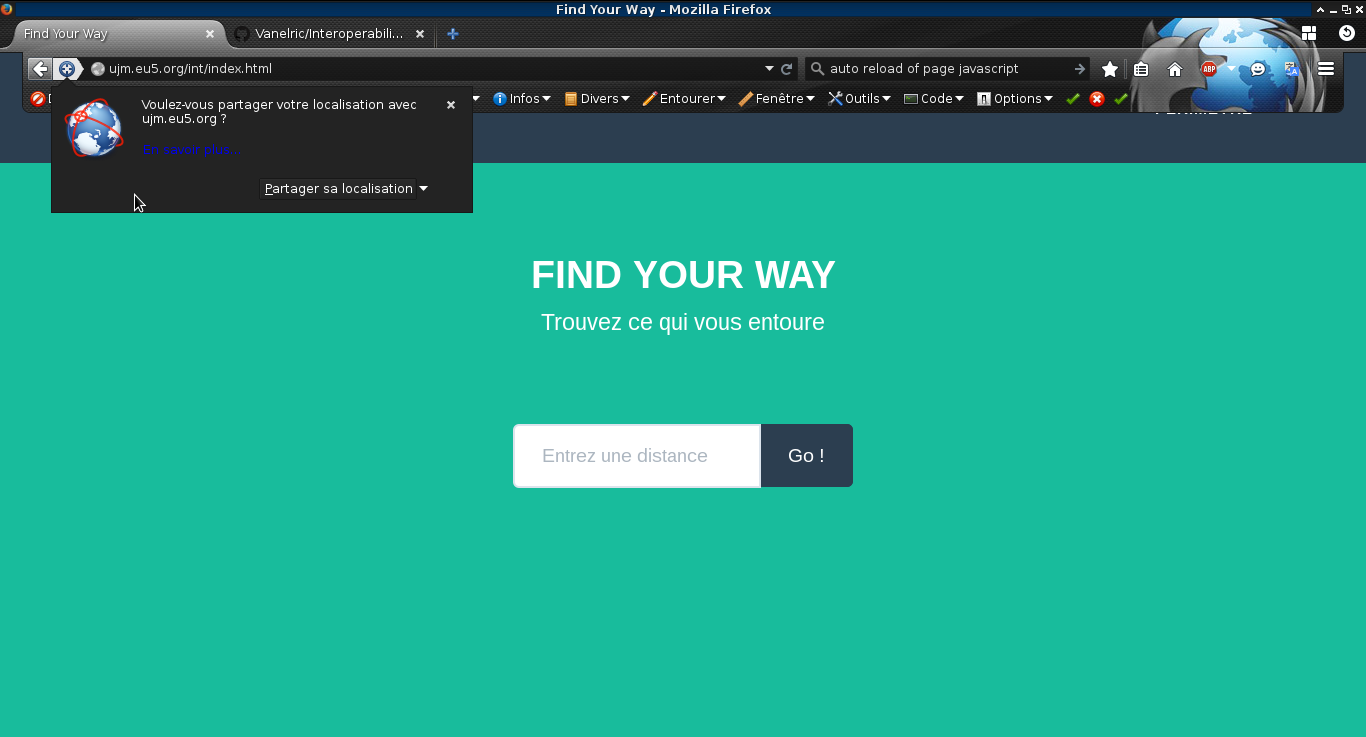
\includegraphics[scale=0.5]{images/accueil_demande.png} %
}%

\newpage
Une fois celle-ci autorisée nous remplissons le champs pour le rayon dans lequel nous cherchons les différents lieux. \\
Puis validons le formulaire en cliquant simplement sur "Go !" \\
{%
\setlength{\fboxsep}{0pt}%
\setlength{\fboxrule}{2pt}%
\fbox{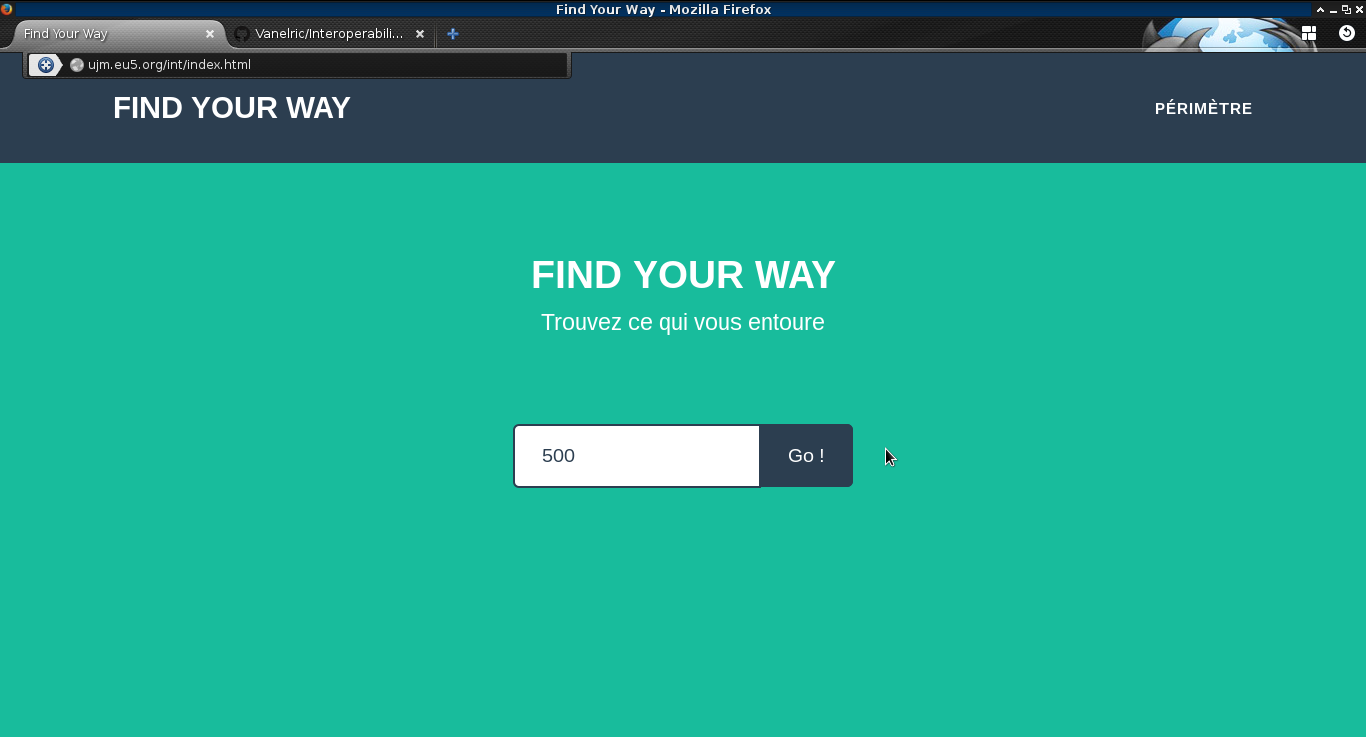
\includegraphics[scale=0.5]{images/accueil_rempli.png} %
}%

\newpage
\section{\uuline{Le choix}}

Une fois le clic effectué, nous somme redirigé sur la page qui nous montre la carte. \\
Nous avons donc une liste non-exhaustive des lieux qui nous entourent ( google map limitant à 20 curseurs sur la carte ). \\
{%
\setlength{\fboxsep}{0pt}%
\setlength{\fboxrule}{2pt}%
\fbox{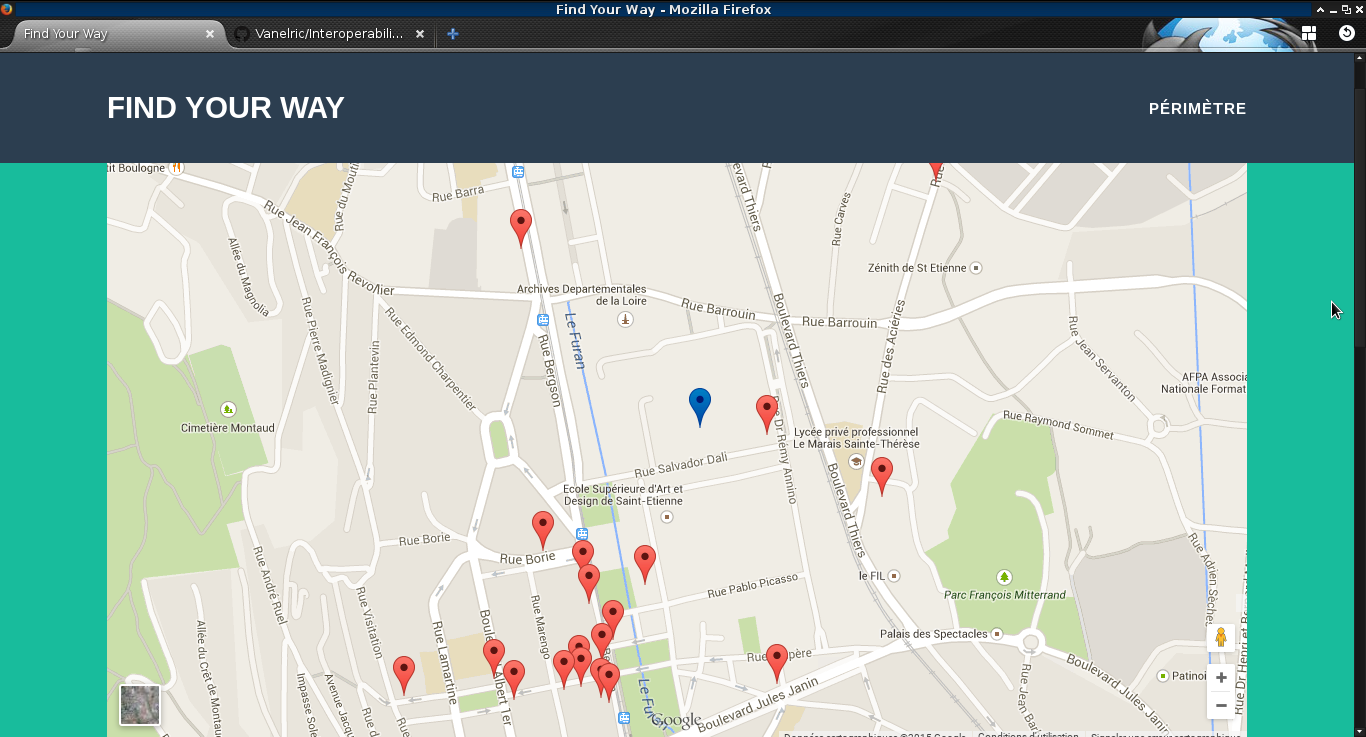
\includegraphics[scale=0.5]{images/map.png}%
}%

\newpage
En "scrollant" alors sur la page nous pouvons accéder aux choix. \\
Par exemple regardons les bars autour de la faculté des sciences (campus Carnot). \\
{%
\setlength{\fboxsep}{0pt}%
\setlength{\fboxrule}{2pt}%
\fbox{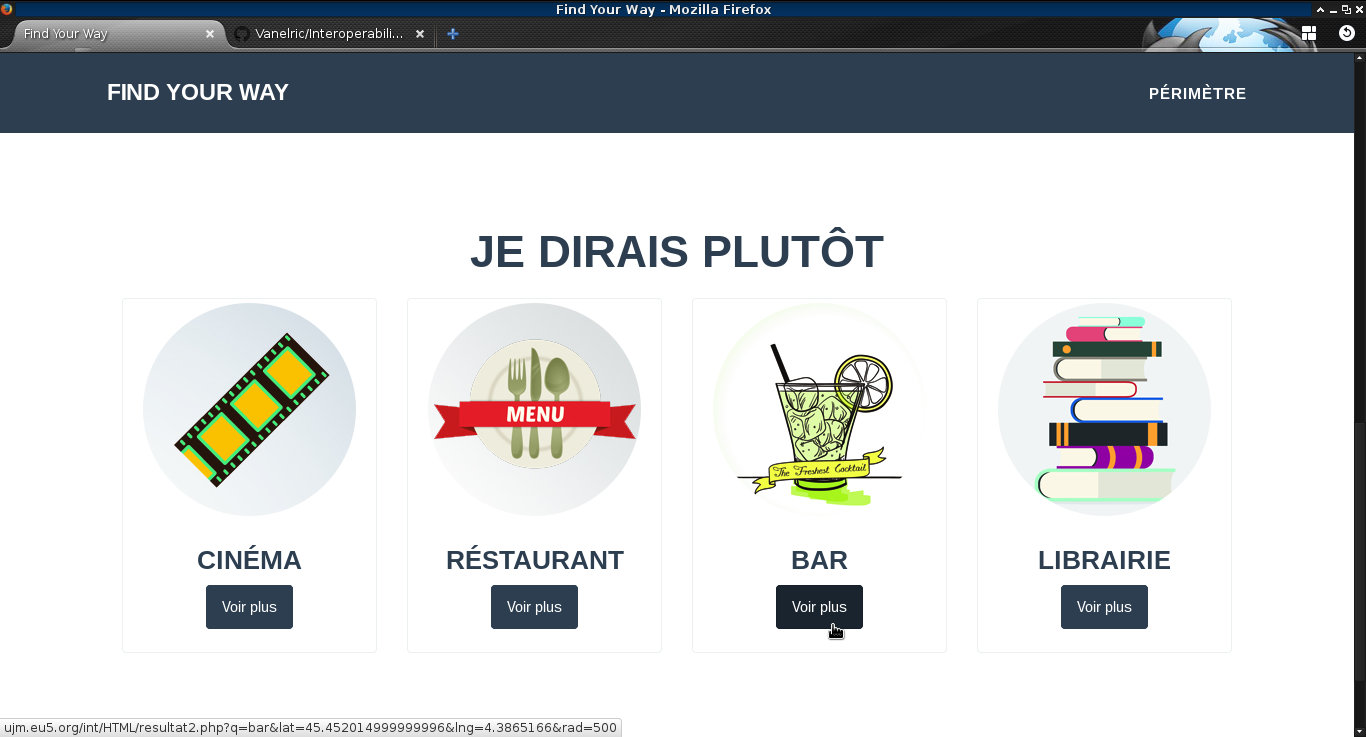
\includegraphics[scale=0.5]{images/choix.png} %
}%

\newpage
\section{\uuline{Vote et affichage}}

Ici nous voici enfin sur la liste des commerces proches de nous, la distance ainsi que l'adresse est affichée. \\
Nous pouvons également cliquer sur le nom du commerce pour avoir plus d'informations sur celui-ci. \\
Par exemple dans les cinémas, la liste des films ainsi que leurs horaires de diffusions seront indiqués. \\
Dans la partie "Librairie" une liste des nouveaux livres sera affichée. \\
Enfin dans la partie "Bar" une liste des cocktails de saisons sera affichée avec leurs ingrédients. \\
{%
\setlength{\fboxsep}{0pt}%
\setlength{\fboxrule}{2pt}%
\fbox{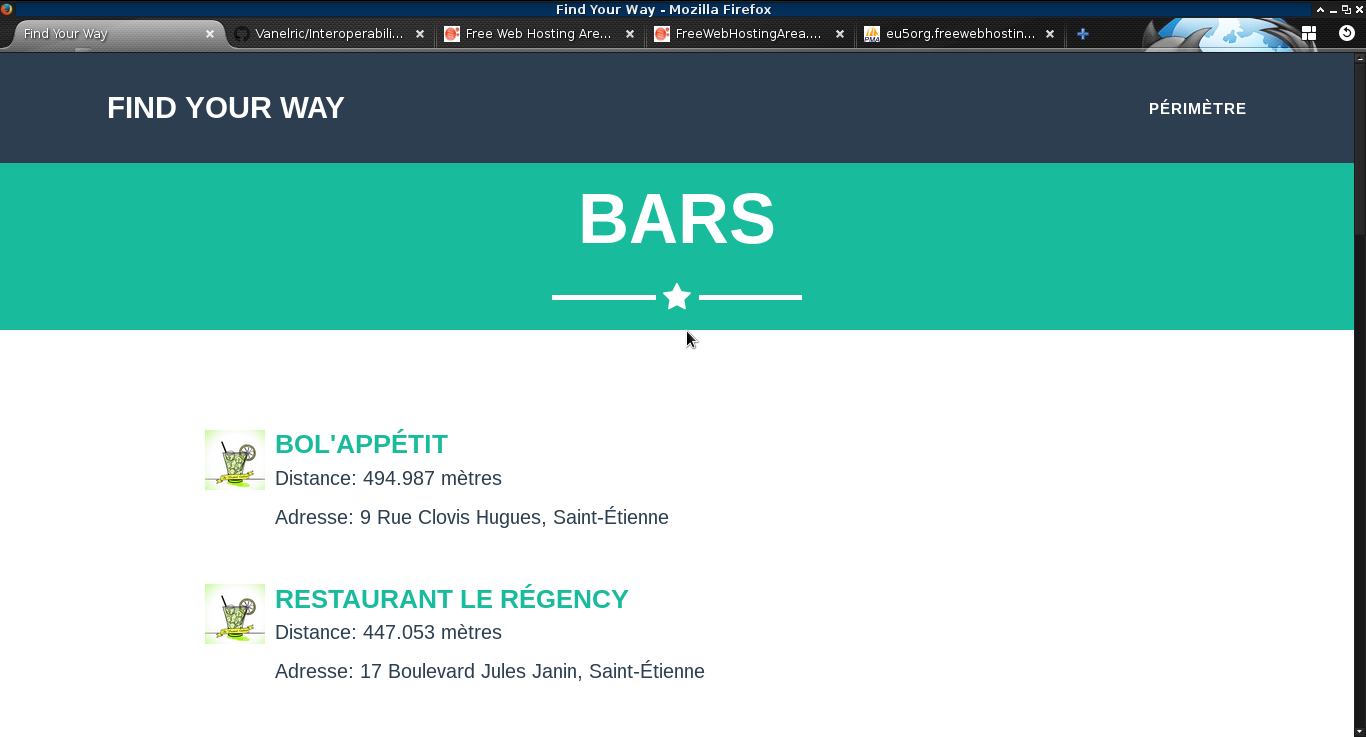
\includegraphics[scale=0.5]{images/bar_liste.png} %
}%

\newpage
Nous voici, après avoir cliqué sur le titre du bar "Bol' Appétit" une liste de cocktail mais également la possibilité de voter pour ce bar. \\
Afin d'indiquer aux autres si celui-ci est bien ou pas. \\
{%
\setlength{\fboxsep}{0pt}%
\setlength{\fboxrule}{2pt}%
\fbox{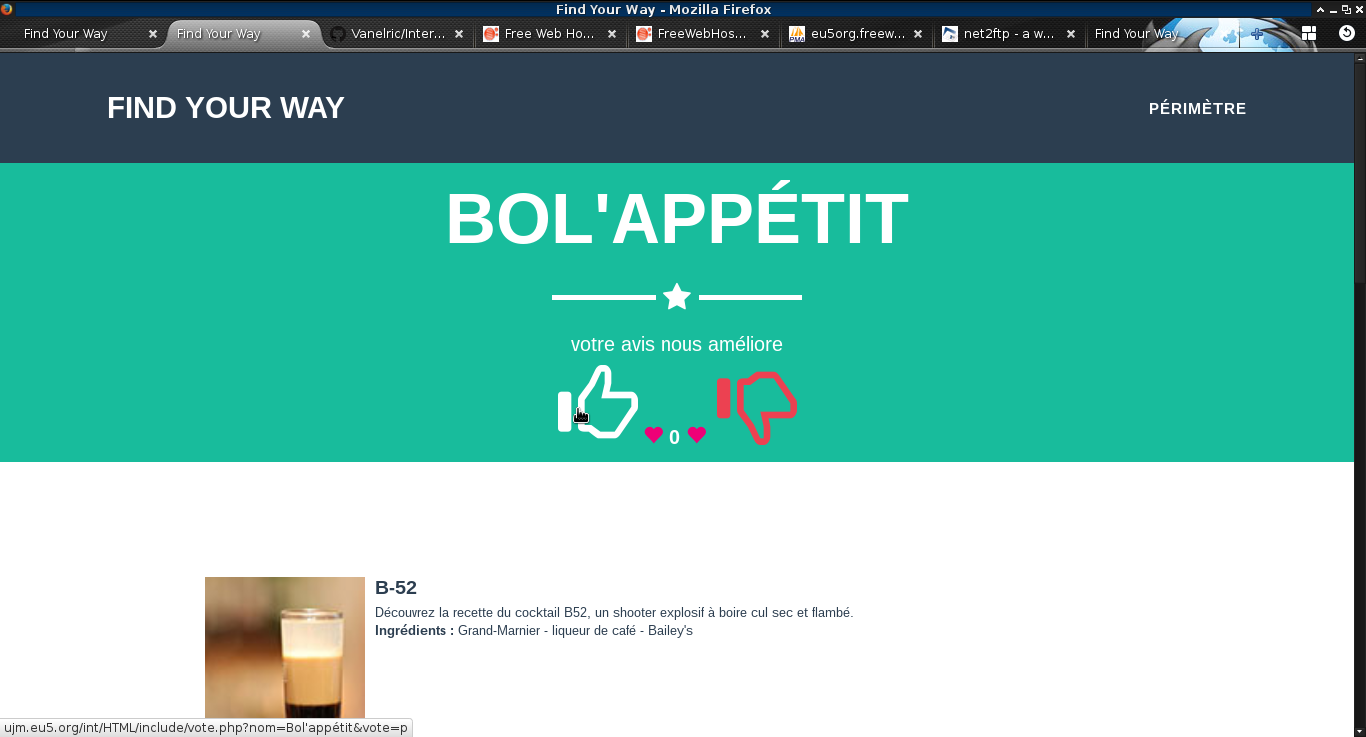
\includegraphics[scale=0.5]{images/cocktail.png} %
}%

\newpage
Une fois le vote effectué, les boutons pour le vote sont cachés, ainsi seul le total de vote reste affiché.
Un vote plus augmentera de 1 le nombre de "j'aime" \\
Un vote négative appliquera -1 sur le total de personne ayant aimé ce bar. \\

Un mauvais bar aura dès lors une note négative. \\
{%
\setlength{\fboxsep}{0pt}%
\setlength{\fboxrule}{2pt}%
\fbox{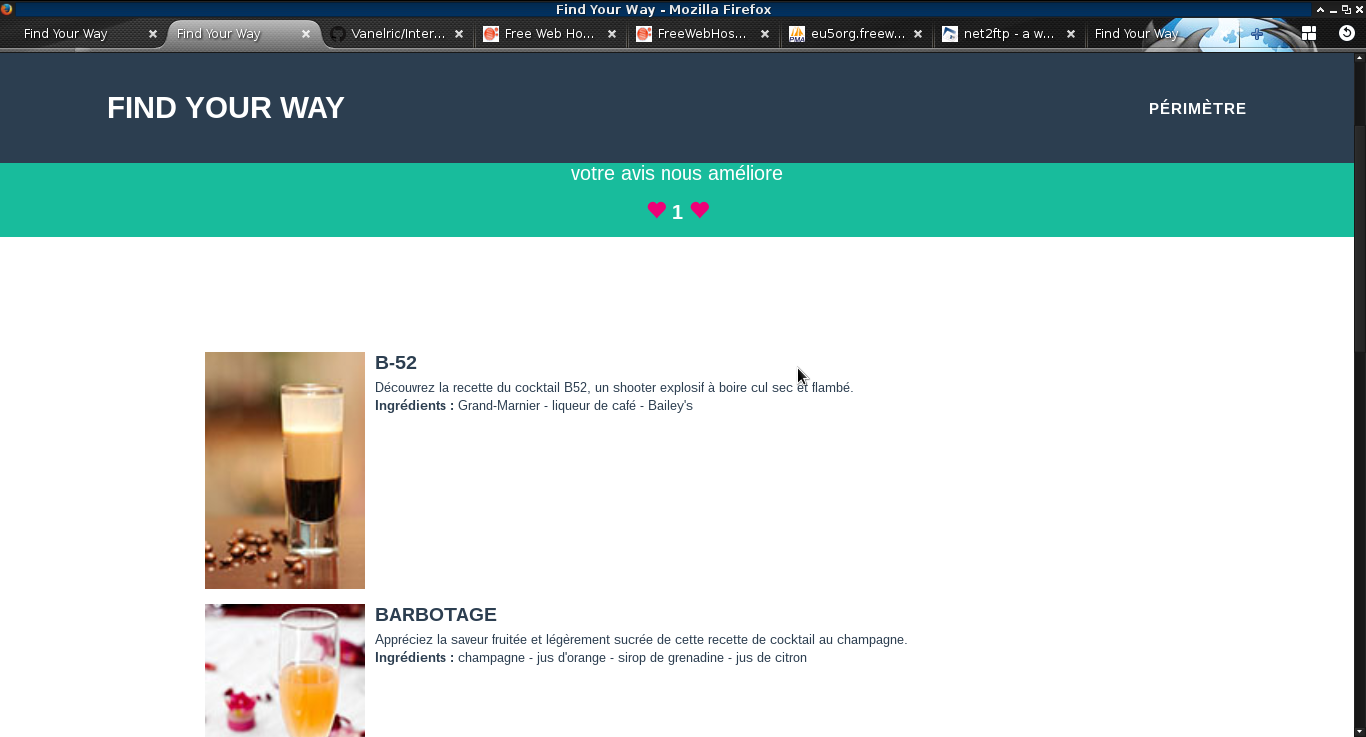
\includegraphics[scale=0.5]{images/vote.png} %
}%

\newpage
\section{\uuline{Ajout de lieu}}

Supposons maintenant que notre lieu favori n'est pas présent dans la liste des bars, ou la liste des librairies etc.. \\
Nous pouvons l'ajouter en cliquant simplement sur le bouton "Ajouter un lieu" , présent en bas de la liste complète d'un thème donné. \\\
un formulaire apparait alors. \\

Nous allons alors ajouter un bar ici nous le nommerons "Carnot Bar" présent à l'adresse de la faculté. \\
Cliquons ensuite sur "Ajouter le lieu".
{%
\setlength{\fboxsep}{0pt}%
\setlength{\fboxrule}{2pt}%
\fbox{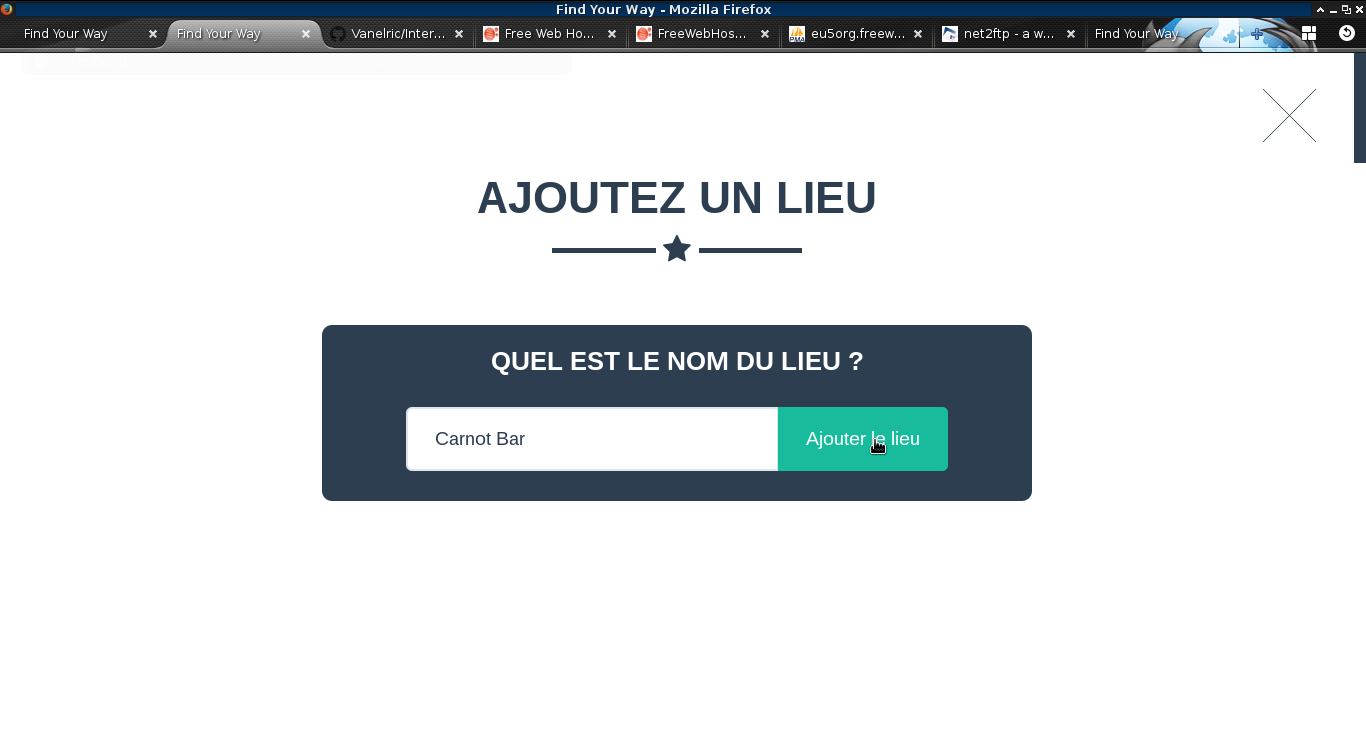
\includegraphics[scale=0.5]{images/ajout_lieu.png} %
}%

\newpage
Un message apparait alors pour nous indiquer que le lieu à bien été ajouté. \\
Dans le cas où le lieu existe déjà un message nous indique que "Le lieu existe déjà". \\
{%
\setlength{\fboxsep}{0pt}%
\setlength{\fboxrule}{2pt}%
\fbox{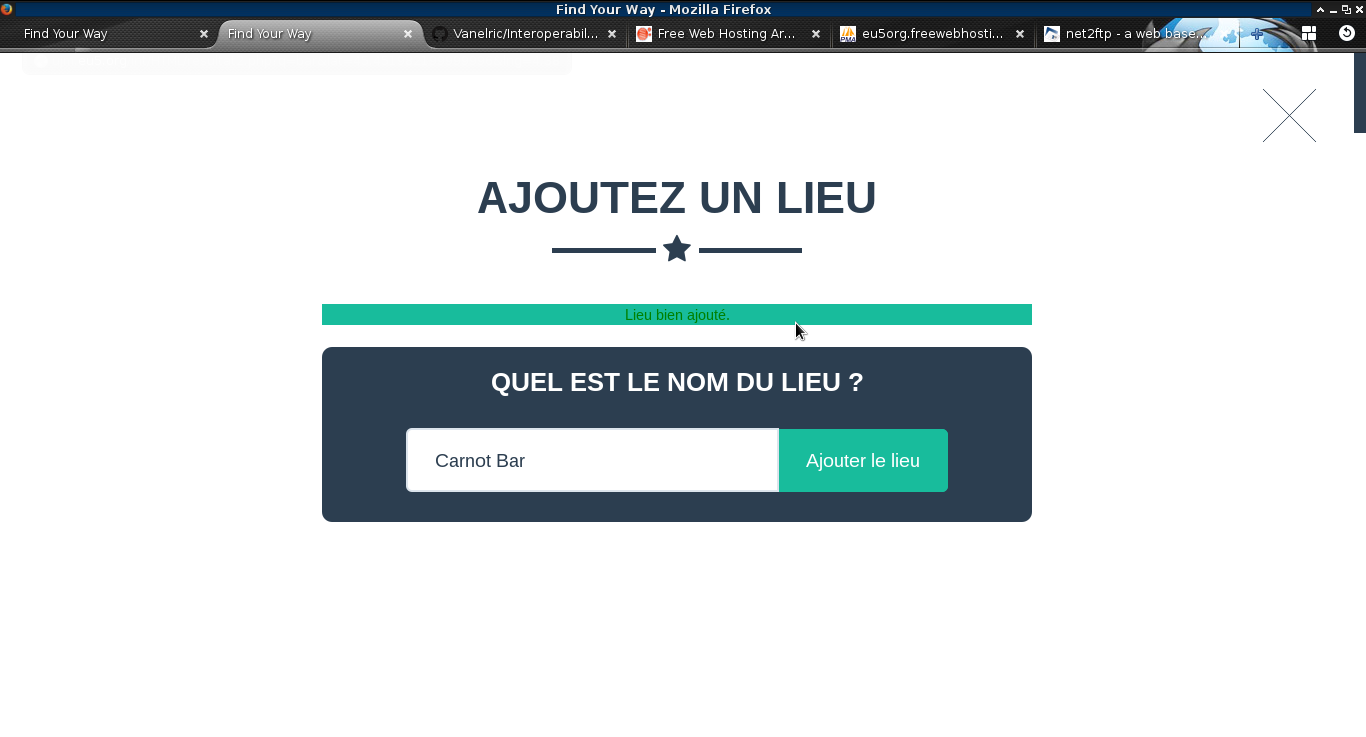
\includegraphics[scale=0.5]{images/good_ajout.png} %
}%

\newpage
Puis après 5 secondes, la page se recharge automatiquement pour nous afficher la nouvelle liste avec le lieu ajouté. \\
{%
\setlength{\fboxsep}{0pt}%
\setlength{\fboxrule}{2pt}%
\fbox{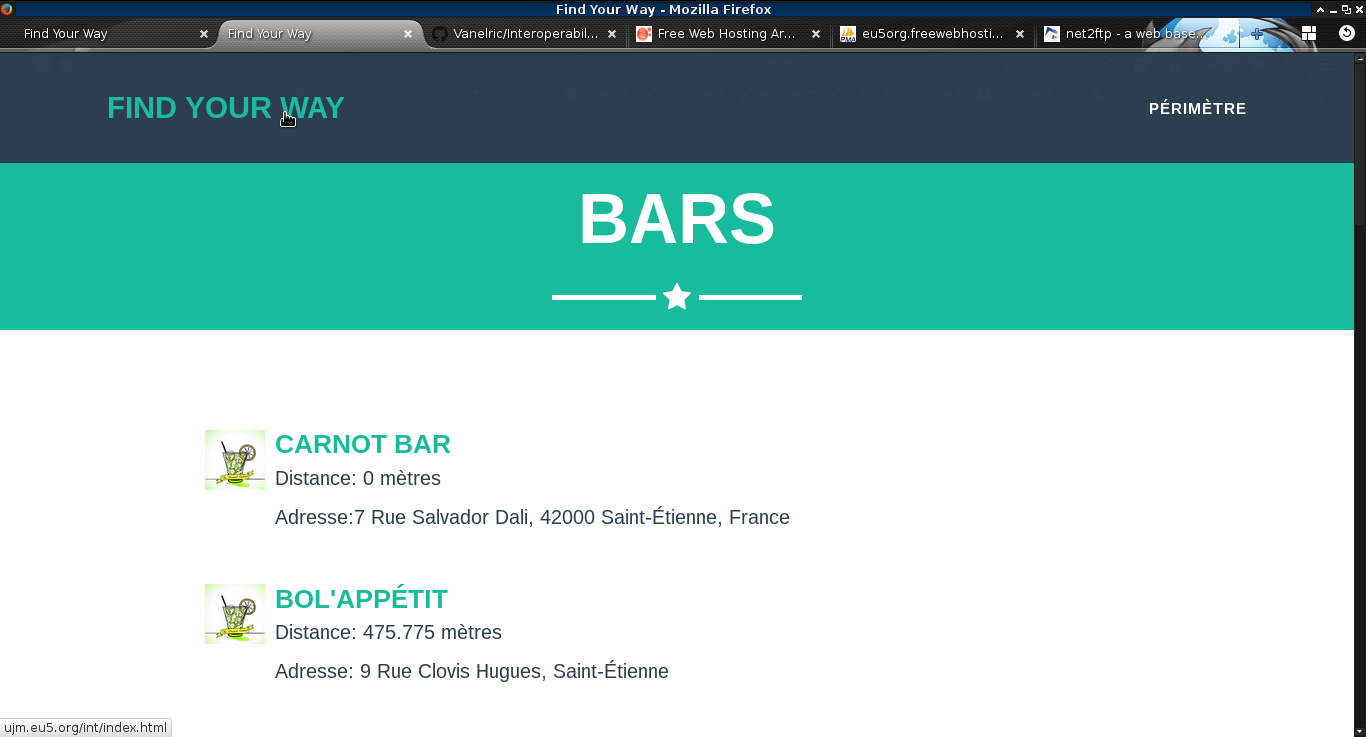
\includegraphics[scale=0.5]{images/carnot_ajouter.png} %
}%

\end{document}